\documentclass[border=1mm]{standalone}
% \documentclass{article}
\usepackage[margin=2.5cm]{geometry}

\usepackage{graphicx,tikz,tikz-layers,amsmath} 
\usetikzlibrary{decorations.markings,calc,positioning,arrows,shapes.geometric,arrows.meta}

\colorlet{myred}{red!80!black}
\colorlet{myblue}{blue!80!black}
\colorlet{mybluee}{myblue!80!black}
\colorlet{mygreen}{green!60!black}
\colorlet{myorange}{orange!70!red!60!black}
\colorlet{mydarkred}{red!20!black}
\colorlet{mydarkblue}{blue!40!black}
\colorlet{mydarkgreen}{green!20!black}




\begin{document}

\resizebox{\textwidth}{!}{
\tikz[font=\footnotesize,scale=1, every node/.style={outer sep=0pt, inner sep=0pt,align=center}, w/.style={minimum width=#1},h/.style={minimum height=#1},s/.style={minimum size=#1}, eu/.style={shorten >=#1},ed/.style={shorten <=#1}, line join=round]
{
\tikzset{>={Latex[length=1.75mm,width=1.25mm]}}
% \tikzset{>={Latex[length=2mm,width=1.5mm]}}

% Blocks
\node[draw, s=1cm, fill=mygreen!40] (g1) {};

\node[draw, circle, s=1cm, right=.5cm of g1, rounded corners=1mm, fill=myblue!20] (h0) {$h_0$};
\node[w=1.25cm, h=1cm, below=.5cm of g1, rounded corners=0mm] (cnn) {CNN};
\begin{scope}[on behind layer]
\draw[fill=mygreen!20] (cnn.south west)--(cnn.south east)--($(cnn.north east)+(-.15,0)$)--($(cnn.north west)+(.15,0)$)--cycle;
\end{scope}

\node[draw, circle, s=1cm, right=2cm of h0, rounded corners=1mm, fill=myblue!20] (h1) {$h_1$};

\node[draw, s=1cm, above=.5cm of h0, label={[label distance=1mm]above:$\alpha_1$}] (g2) {};
\node[draw, s=1cm, above=.5cm of h1, xshift=-.7cm, label={[label distance=1mm]above:$\alpha_2$}] (g3) {};
\node[draw, circle, s=1cm, above=.5cm of h1, xshift=.7cm, rounded corners=1mm, fill=myred!20] (py1) {$p(y_1)$};
\node[draw, circle, s=1cm, below=.5cm of h1, xshift=-.7cm, rounded corners=1mm, fill=mygreen!20] (z1) {$z_1$};
\node[draw, circle, s=1cm, below=.5cm of h1, xshift=.7cm, rounded corners=1mm, fill=myorange!20] (y0) {$y_0$};

% Image
\node[draw, below=.5cm of cnn] (im1) {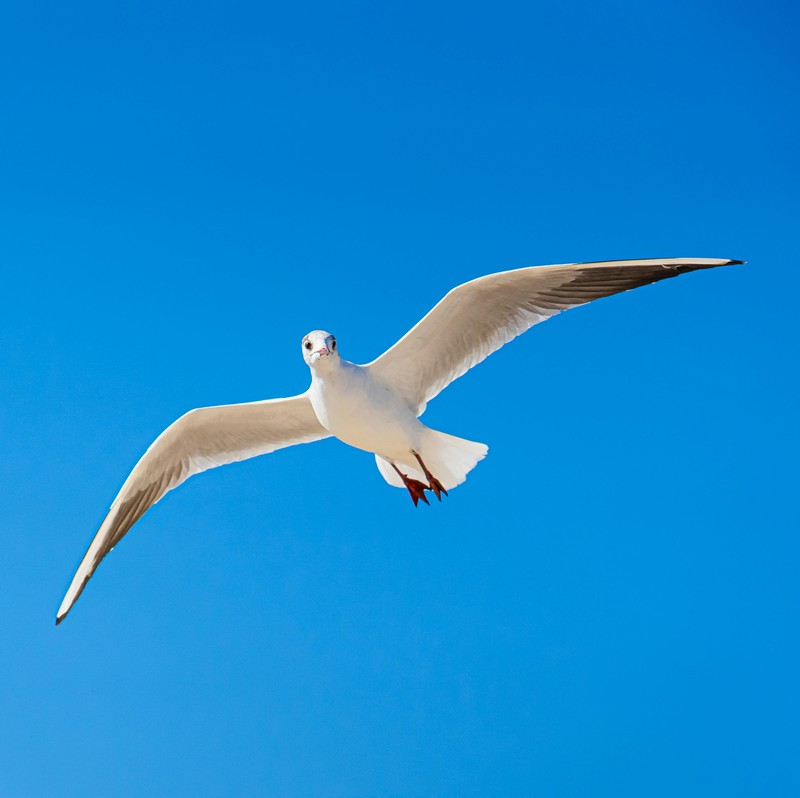
\includegraphics[width=1.25cm]{tikz/chapter7 - Show, Attend and Tell.jpg}};

% Arrows
\draw[->] (im1)--(cnn);
\draw[->] (cnn)--(g1);
\draw[->] (g1)--(h0);
\draw[->] (h0)--(h1);
\draw[->] (h0)--(g2);
\draw[->] (h1.100)--++(0,.2) -| (g3);
\draw[->] (h1.80)--++(0,.2) -| (py1);
\draw[->] (z1.north)--++(0,.2) -| (h1.-110);
\draw[->] (y0.north)--++(0,.2) -| (h1.-70);
\draw[->, myred] (g1.-10) to[out=-45, in=180] (z1.200);
\begin{scope}[on behind layer]
\draw[->, myred] (g2.0) to[out=-20, in=180, looseness=.8] node[pos=.468,circle, fill=white, inner sep=1pt] {} (z1.180);    
\end{scope}

\draw[->] (h1)--+(2,0);

% Titles
\node[below=2mm] at ($(z1.south)!.5!(y0.south)$) {Context Vector};
\node[above=5mm of g1,align=center, xshift=-3mm] {Feature Map\\$14\times14\times512$};

% Grid
\foreach \i in {1,2,3}
\draw 
($(g\i.north west)!.333!(g\i.north east)$)--($(g\i.south west)!.333!(g\i.south east)$)
($(g\i.north west)!.666!(g\i.north east)$)--($(g\i.south west)!.666!(g\i.south east)$)
($(g\i.north west)!.333!(g\i.south west)$)--($(g\i.north east)!.333!(g\i.south east)$)
($(g\i.north west)!.666!(g\i.south west)$)--($(g\i.north east)!.666!(g\i.south east)$);

%---------------------------Middle shape------------------------
\begin{scope}[xshift=10cm]
% Blocks
\node[draw, s=1cm, fill=mygreen!40] (g1) {};

\node[draw, circle, s=1cm, right=.5cm of g1, rounded corners=1mm, fill=myblue!20] (h0) {$h_0$};
\node[w=1.25cm, h=1cm, below=.5cm of g1, rounded corners=0mm] (cnn) {CNN};
\begin{scope}[on behind layer]
\draw[fill=mygreen!20] (cnn.south west)--(cnn.south east)--($(cnn.north east)+(-.15,0)$)--($(cnn.north west)+(.15,0)$)--cycle;
\end{scope}
\node[draw, circle, s=1cm, right=2cm of h0, rounded corners=1mm, fill=myblue!20] (h1) {$h_1$};

\node[draw, s=1cm, above=.5cm of h0, label={[label distance=1mm]above:$\alpha_1$}] (g2) {};
\node[draw, s=1cm, above=.5cm of h1, xshift=-.7cm, label={[label distance=1mm]above:$\alpha_2$}] (g3) {};
\node[draw, circle, s=1cm, above=.5cm of h1, xshift=.7cm, rounded corners=1mm, fill=myred!20] (py1) {$p(y_1)$};
\node[draw, circle, s=1cm, below=.5cm of h1, xshift=-.7cm, rounded corners=1mm, fill=mygreen!20] (z1) {$z_1$};
\node[draw, circle, s=1cm, below=.5cm of h1, xshift=.7cm, rounded corners=1mm, fill=myorange!20] (y0) {$y_0$};

\node[draw, circle, s=1cm, right=1cm of y0, rounded corners=1mm, fill=mygreen!20] (z2) {$z_2$};
% Image
\node[draw, below=.5cm of cnn] (im1) {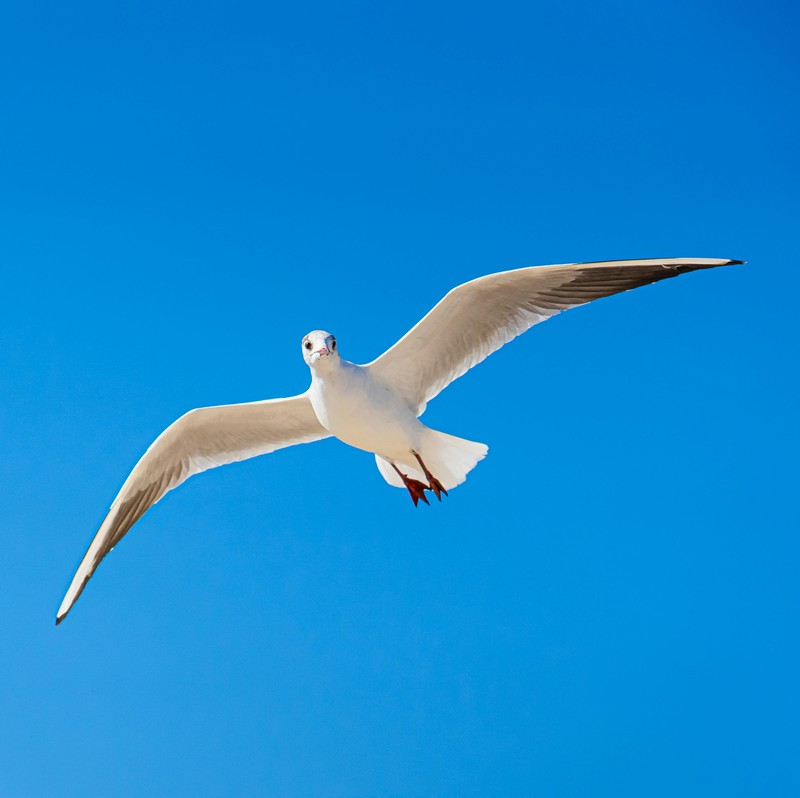
\includegraphics[width=1.25cm]{tikz/chapter7 - Show, Attend and Tell.jpg}};

% Arrows
\draw[->] (im1)--(cnn);
\draw[->] (cnn)--(g1);
\draw[->] (g1)--(h0);
\draw[->] (h0)--(h1);
\draw[->] (h0)--(g2);
\draw[->] (h1.100)--++(0,.2) -| (g3);
\draw[->] (h1.80)--++(0,.2) -| (py1);
\draw[->] (z1.north)--++(0,.2) -| (h1.-110);
\draw[->] (y0.north)--++(0,.2) -| (h1.-70);
\draw[->, myred] (g1.-10) to[out=-45, in=-150, looseness=1.3] (z2.-90);

\begin{scope}[on behind layer]
\draw[->, myred] (g3.0) to[out=-30, in=180, looseness=.8] node[pos=.273,circle, fill=white, inner sep=1pt] {} node[pos=.443,circle, fill=white, inner sep=1pt] {} (z2.180);   
\end{scope}

\draw[->] (h1)--+(2,0);

% Titles
\node[below=2mm] at ($(z1.south)!.5!(y0.south)$) {Context Vector};
\node[above=5mm of g1,align=center, xshift=-3mm] {Feature Map\\$14\times14\times512$};

% Grid
\foreach \i in {1,2,3}
\draw 
($(g\i.north west)!.333!(g\i.north east)$)--($(g\i.south west)!.333!(g\i.south east)$)
($(g\i.north west)!.666!(g\i.north east)$)--($(g\i.south west)!.666!(g\i.south east)$)
($(g\i.north west)!.333!(g\i.south west)$)--($(g\i.north east)!.333!(g\i.south east)$)
($(g\i.north west)!.666!(g\i.south west)$)--($(g\i.north east)!.666!(g\i.south east)$);
\end{scope}


%---------------------------Shape on the right hand side------------------------
\begin{scope}[xshift=3.7cm, yshift=-7.2cm]
% Blocks
\node[draw, s=1cm, fill=mygreen!40] (g1) {};

\node[draw, circle, s=1cm, right=.5cm of g1, rounded corners=1mm, fill=myblue!20] (h0) {$h_0$};
\node[w=1.25cm, h=1cm, below=.5cm of g1, rounded corners=0mm] (cnn) {CNN};

\begin{scope}[on behind layer]
\draw[fill=mygreen!20] (cnn.south west)--(cnn.south east)--($(cnn.north east)+(-.15,0)$)--($(cnn.north west)+(.15,0)$)--cycle;
\end{scope}
\node[draw, circle, s=1cm, right=2cm of h0, rounded corners=1mm, fill=myblue!20] (h1) {$h_1$};

\node[draw, s=1cm, above=.5cm of h0, label={[label distance=1mm]above:$\alpha_1$}] (g2) {};
\node[draw, s=1cm, above=.5cm of h1, xshift=-.7cm, label={[label distance=1mm]above:$\alpha_2$}] (g3) {};
\node[draw, circle, s=1cm, above=.5cm of h1, xshift=.7cm, rounded corners=1mm, fill=myred!20] (py1) {$p(y_1)$};
\node[draw, circle, s=1cm, below=.5cm of h1, xshift=-.7cm, rounded corners=1mm, fill=mygreen!20] (z1) {$z_1$};
\node[draw, circle, s=1cm, below=.5cm of h1, xshift=.7cm, rounded corners=1mm, fill=myorange!20] (y0) {$y_0$};

\node[draw, circle, s=1cm, right=3cm of h1, rounded corners=1mm, fill=myblue!20] (h2) {$h_2$};
\node[draw, s=1cm, above=.5cm of h2, xshift=-.7cm, label={[label distance=1mm]above:$\alpha_2$}] (g4) {};
\node[draw, circle, s=1cm, above=.5cm of h2, xshift=.7cm, rounded corners=1mm, fill=myred!20] (py2) {$p(y_2)$};
\node[draw, circle, s=1cm, below=.5cm of h2, xshift=-.7cm, rounded corners=1mm, fill=mygreen!20] (z2) {$z_2$};
\node[draw, circle, s=1cm, below=.5cm of h2, xshift=.7cm, rounded corners=1mm, fill=myorange!20] (y1) {$y_1$};

% Image
\node[draw, below=.5cm of cnn] (im1) {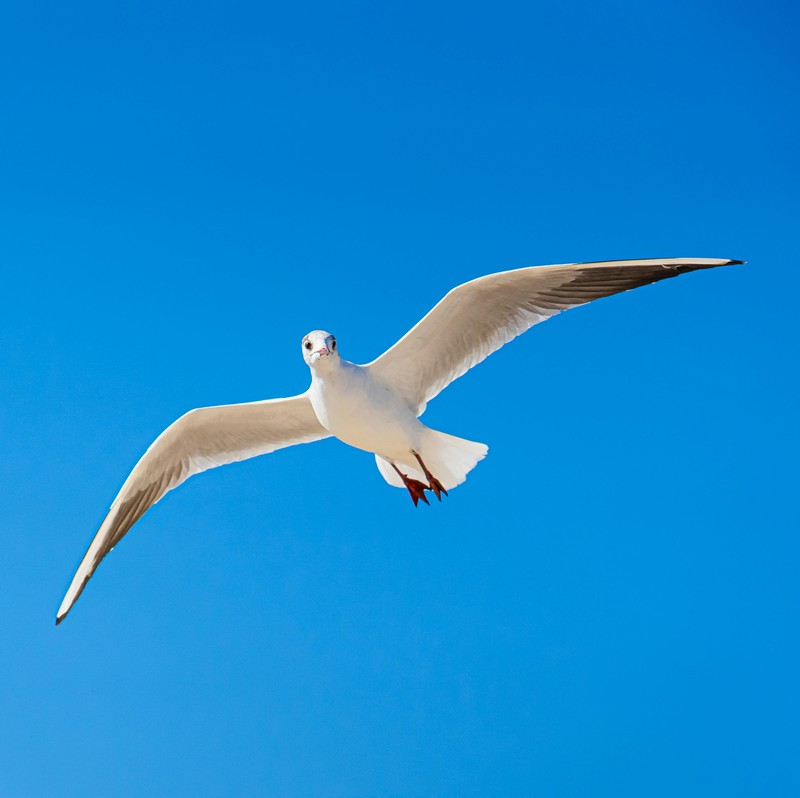
\includegraphics[width=1.25cm]{tikz/chapter7 - Show, Attend and Tell.jpg}};

% Arrows
\draw[->] (im1)--(cnn);
\draw[->] (cnn)--(g1);
\draw[->] (g1)--(h0);\draw[->] (g1)--(h0);
\draw[->] (h0)--(h1);
\draw[->] (h0)--(g2);
\draw[->] (h1.100)--++(0,.2) -| (g3);
\draw[->] (h1.80)--++(0,.2) -| (py1);
\draw[->] (z1.north)--++(0,.2) -| (h1.-110);
\draw[->] (y0.north)--++(0,.2) -| (h1.-70);

\draw[->, myred] (py1.-70) to[out=-70, in=-120, looseness=1.3] node[pos=.145,circle, fill=white, inner sep=1pt] {} (y1.-90);

\draw[->] (h1)--(h2);
\draw[->] (h2.100)--++(0,.2) -| (g4);
\draw[->] (h2.80)--++(0,.2) -| (py2);
\draw[->] (z2.north)--++(0,.2) -| (h2.-110);
\draw[->] (y1.north)--++(0,.2) -| (h2.-70);
\draw[->] (h2)--+(2,0);

% Titles
\node[below=2mm] at ($(z1.south)!.5!(y0.south)$) {$<$START$>$};
\node[above=5mm of g1,align=center, xshift=-3mm] {Feature Map\\$14\times14\times512$};

% Grid
\foreach \i in {1,2,3,4}
\draw 
($(g\i.north west)!.333!(g\i.north east)$)--($(g\i.south west)!.333!(g\i.south east)$)
($(g\i.north west)!.666!(g\i.north east)$)--($(g\i.south west)!.666!(g\i.south east)$)
($(g\i.north west)!.333!(g\i.south west)$)--($(g\i.north east)!.333!(g\i.south east)$)
($(g\i.north west)!.666!(g\i.south west)$)--($(g\i.north east)!.666!(g\i.south east)$);
\end{scope}
}
}

\end{document}